\documentclass{beamer}
\usepackage{beamerthemesplit}
\usepackage{lmodern}
\usepackage{graphicx} 
\usepackage[absolute,overlay]{textpos}

\setbeamercolor{framesource}{fg=black}
\setbeamerfont{framesource}{size=\tiny}

\newcommand{\source}[1]{\begin{textblock*}{4cm}(8.5cm,8.1cm)
	\begin{beamercolorbox}[ht=0.5cm,right]{framesource}
		\usebeamerfont{framesource}\usebeamercolor[fg]{framesource} Source: {#1}
	\end{beamercolorbox}
\end{textblock*}}


\title{Evacuation Bottleneck}
\subtitle{Simulating a Panic on a Cruise Ship}
\author{Johannes Weinbuch, Benedek Vartok}
\date{}

\begin{document}
\frame{\titlepage}

%Johannes
\begin{frame}
	\frametitle{Outline}
	\tableofcontents
\end{frame}

\section{Introduction}

%Johannes
\begin{frame}
	\frametitle{Our Research Object}
	\begin{columns}
		\begin{column}{5cm}
			\begin{itemize}
				\item Costa Voyager
				\item Capacity: 836 passengers
				\item 8 Rescue Boats
				\item In distress at sea in 2005
			\end{itemize}
		\end{column}
		\begin{column}{5cm}
			\begin{centering}
				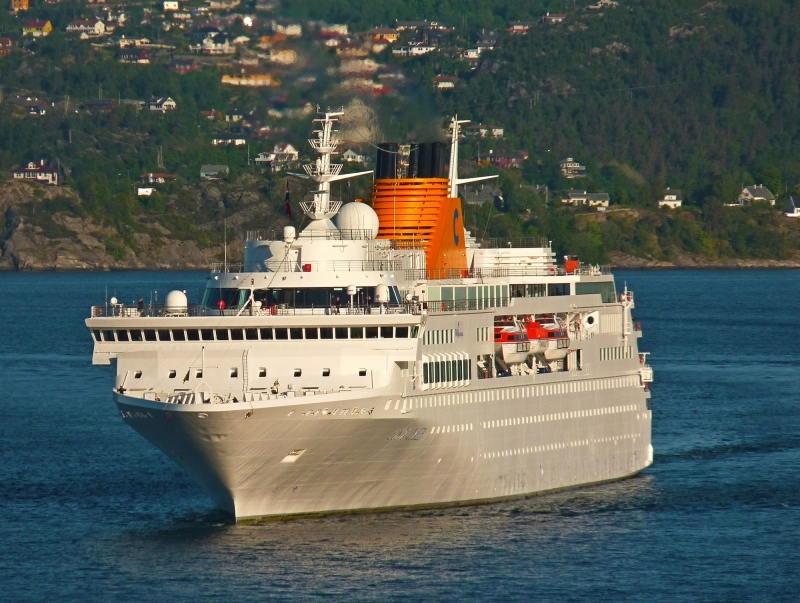
\includegraphics[scale=0.5]{images/costavoyager.jpg}
			\end{centering}
		\end{column}
	\end{columns}
	\source{http://www.shipspotting.com, Picture taken by Roy Batty}
\end{frame}

\section{Our Model}

%Johannes
\subsection{Input}
\begin{frame}
	\frametitle{The Deck Plan}
	\begin{columns}
		\begin{column}{5cm}
			\begin{itemize}
				\item Colormap
					\begin{itemize}
						\item Allows any number of zones
					\end{itemize}
				\item Scaling
				\item Greatly simplyfied
			\end{itemize}
		\end{column}
		\begin{column}{2.5cm}
			\begin{center}
				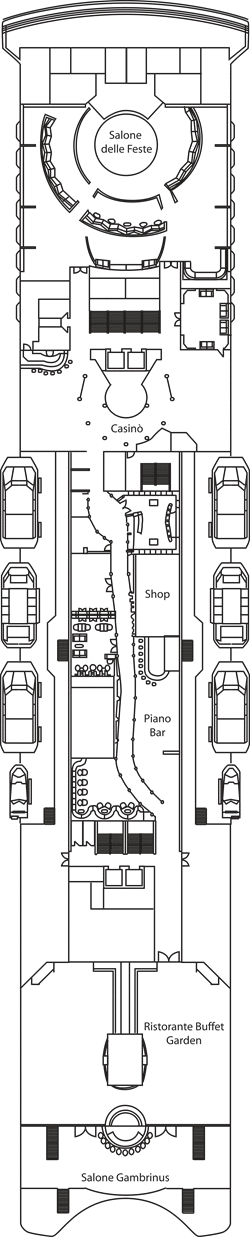
\includegraphics[height=5cm]{images/deckbefore.png}
			\end{center}
		\end{column}
		\begin{column}{2.5cm}
			\begin{center}
				
\includegraphics[height=5cm]{images/deckafter.png}
			\end{center}
		\end{column}
	\end{columns}
	\source{http://www.kreuzfahrtberater.de}
\end{frame}

\begin{frame}
	\begin{itemize}
		\item TODO: config file
	\end{itemize}
\end{frame}

\subsection{Forces}
\begin{frame}
	\begin{itemize}
		\item TODO: desired, agent-, wall-forces
	\end{itemize}
\end{frame}

\subsection{Filled Exits}
\begin{frame}
	\begin{itemize}
		\item TODO: exits
	\end{itemize}
\end{frame}

\section{Implementation}

\begin{frame}
	\begin{itemize}
		\item TODO: we reused code from Multilevel Evacuation
	\end{itemize}
\end{frame}

\section{Results}

\subsection{Passenger Distribution}
\begin{frame}
	\frametitle{Distribution of the Agents to the Exits}
	\begin{itemize}
		\item The distribution depends strongly on the geometry of the ship.
		\item There was no case where the agents really distributed over the exits
		\begin{itemize}
			\item Weakness in the model
			\item More realistic: go for the shortest individual evacuation time
		\end{itemize}
	\end{itemize}
\end{frame}

\subsection{Panic Level}
\begin{frame}
	\begin{itemize}
		\item TODO: more plots and explanations
	\end{itemize}
\end{frame}

\subsection{Summary and Outlook}
\begin{frame}
	\begin{itemize}
		\item TODO: tell how good and/or bad we did
	\end{itemize}
\end{frame}

\section{Outtakes}

\begin{frame}
	\begin{itemize}
		\item TODO: MATLAB -- how we love it!
	\end{itemize}
\end{frame}

\end{document}
